%!TEX root = main.tex
\section{Introduction\label{sec:intro}}
%\todo[inline]{Distinguish b/w bounding box and segmentation and use consistent terminology}
\par The goal of visual scene understanding is to enable computers to achieve high-level comprehension from images or videos. While object localization and detection identifies \textit{where} an object is in the image, object segmentation provides rich information regarding \textit{what} the object looks like. Precise, instance-level object segmentation is crucial for identifying and/or tracking objects in a variety of real-world emergent applications of autonomy, including robotics and autonomous vehicles, surveillance, image organization and retrieval, and medicine~\cite{Irshad2014,Yamaguchi2012}.
%providing a more fine-grained object representation in automated system in with visual inputs, as seen in application such as robotics/autonomous vehicles (CITE),  object parsing \cite{Yamaguchi2012} and biomedical image segmentation \cite{Irshad2014}.
Unfortunately, at present, vision-based object segmentation algorithms often suffer from oversegmented regions and perform poorly for occluded (hidden) objects~\cite{Torralba2010}, for cluttered images with many objects~\cite{Russakovsky2015}, and under undesirable lighting conditions~\cite{bell15minc}. 
\par To this end, there has been a lot of work on employing crowdsourcing to generate training data for computer vision\techreport{\footnote{Kovashka et al. (\citeyear{AdrianaKovashka2016}) is a recent survey on the topic}}. In particular, a number of popular computer vision datasets involve fine-grained segmentation derived from crowdsourcing, including Pascal-VOC~\cite{Everingham15}, LabelMe~\cite{Torralba2010}, OpenSurfaces~\cite{bell15minc}, and MS-COCO~\cite{Lin2012}.
Indeed, fine-grained segmentations are more valuable than more coarse-grained approaches: Kovashka et al. (\citeyear{AdrianaKovashka2016}) state that {\em ``detailed annotations enable the development and evaluation of computer vision algorithms that are able to understand the image on a much finer level than what is possible with just simple binary image-level annotations or with rough bounding box-level localization.''}
\begin{figure}[ht!]
	\centering%, trim=2cm 5cm 1cm 5cm]
	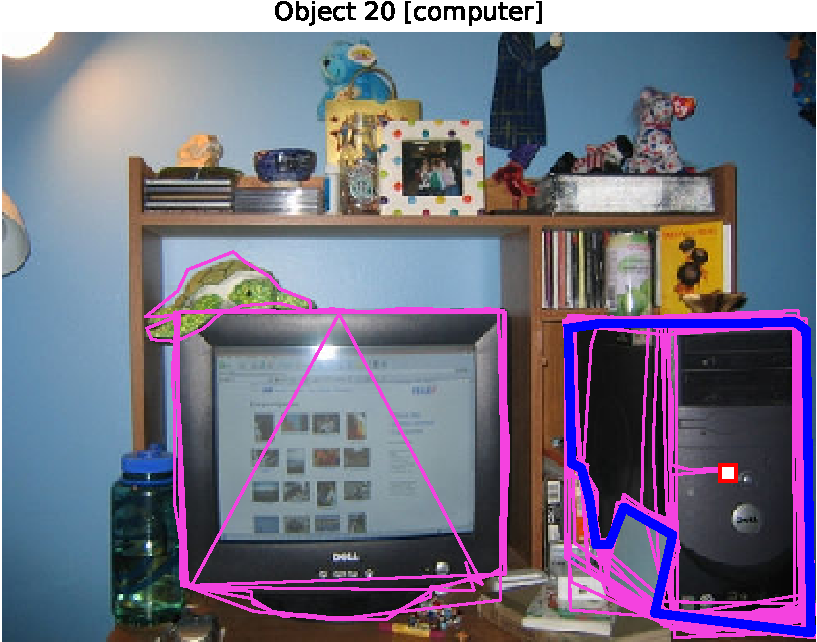
\includegraphics[width=.31\textwidth]{plots/bb_object_20.pdf}
	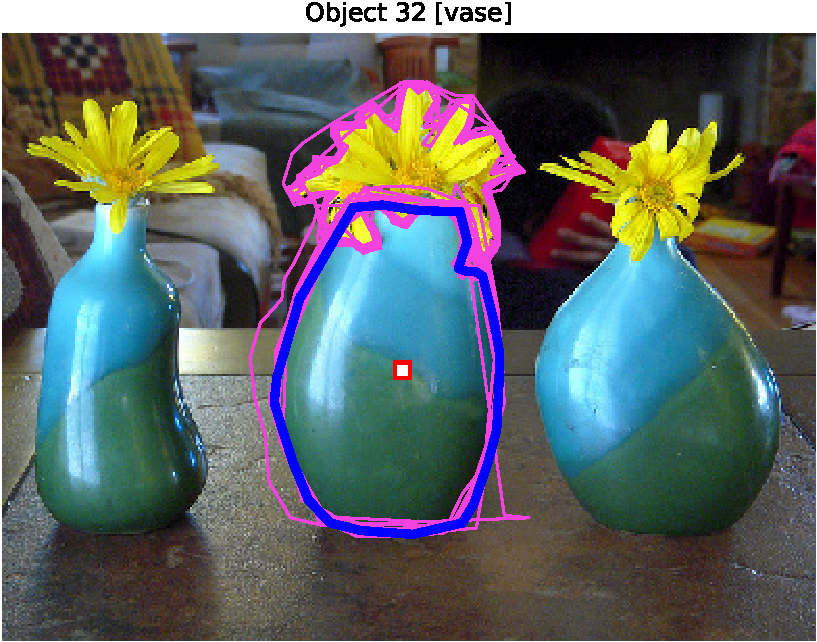
\includegraphics[width=.31\textwidth]{plots/bb_object_32.pdf}
	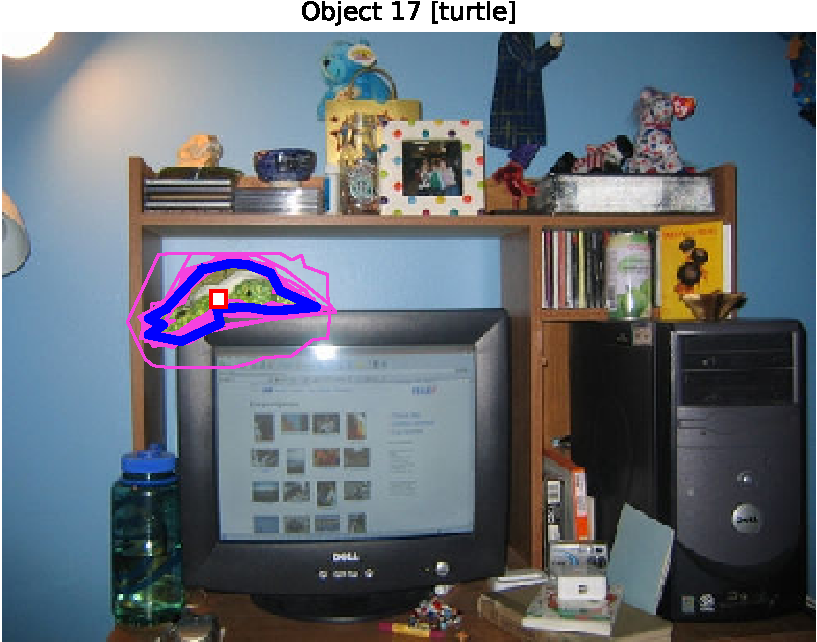
\includegraphics[width=.31\textwidth]{plots/bb_object_17.pdf}
	\caption{Pink is the segmentation from individual workers. Blue solid line delineates the ground truth. The red boxed pointer indicates the task of interest shown to users. Examples demonstrating common error patterns among crowdsourced image segmentation, including 1) annotations on the wrong semantic object, 2) ambiguity in regional inclusion and exclusion, and 3) imprecision at the object boundary.}
	\label{error_examples}
\end{figure}
\par Unfortunately, the use of crowdsourcing for fine-grained segmentation is rife with challenges. As shown in Figure \ref{error_examples}, workers often (i) make unintentional mistakes while drawing the boundaries, either due to low precision of the image, small area of the object, or lack of drawing skills, (ii) have differing opinions about what constitutes the boundary of an object (e.g., is the stalk of a banana part of the fruit?); (iii) or annotate the wrong object entirely (e.g., drawing a bounding box around a dog when the task requests for one around a car). \dor{make the e.g. lines align with what's in the figure.}
%In addition, semantic segmentation often requires crowdsourced image labels or segmentation to address to question of which portion of the image corresponds to the object\cite{Russakovsky2015,Li2009,Bearman2016}. 
%Crowdsourcing worker responses is noisy\todo[inline]{Akash: cite paper about noisiness of crowd response}. Prior studies (CITE?) and empirical observation of our data on crowdsourcing image segmentation have shown that workers errors can fall under three types: ambiguity (worker response can identify the wrong object)\todo[inline]{one could argue that this is really a detection problem not a segmentation problem}, sloppy (low precision at object boundaries), and tendency to underdraw/overdraw.
% is an important part of achieving better visual scene understanding for many downstream applications 
% understanding contextual information between everyday objects \cite{Lin2014}
%\par In order to deal with these issues, one approach is to employ other workers to verify each segmentation 
%provided for correctness~\cite{Lin2014,Everingham15}. %However, this approach provides no mechanism to fix incorrect
%segmentations that are only slightly incorrect. %Another approach is to ask multiple workers to segment the object,following by a  majority vote at the level of pixels~\cite{xxx}. As we will show in the following, this approach does not work very well because it doesn't take into account individual worker qualities, such as a tendency to over or under-draw segmentations. Furthermore, this approach may also lead to {\em discontinuities}, where a single object may erroneously consist of multiple segments.
\par In order to deal with these challenges, many have employed heuristics indicative of segmentation quality, including the idea that segmentation boundaries with more points are likely to be more precise~\cite{Cabezas2015,Sameki2015,Sorokin2008}.%, to pick the best performing worker segmentation.%statistics to pick between different worker segmentations, such as the number of points on the drawn boundary (more implies that the worker segmented the object more carefully), or the area enclosed (more implies that the worker is less likely to have missed some key portions of the object). 
While this approach does enable us to identify the more diligent workers and their annotations, since it is simply picking one ``best'' bounding box based on these heuristics as the solution, it ends up discarding the majority of the worker responses. 
%\todo[inline]{A diagram conveying the intuition of tiles, picking one bounding box, or doing majority voteish stuff would be really nice to set the stage.}
\agp{Comment on whether the focus should be evaluation or new algos (i.e. aggregation based methods)}
Instead, in this paper, we introduced the notion of an {\em aggregation-based} approach capable of incorporating portions of responses from different workers into an overall segmentation.
By overlaying the segmentations from workers on top of each other, we can decompose the image into non-overlapping tiles,
where each tile has some workers who believe this tile belongs to the object, and others who do not.
At this point, we can treat each tile as an independent boolean question, deriving an answer from a worker---does
this tile belong to the object or not, following which we may be able to apply Expectation-Maximization (EM)~\cite{Dawid1979}
to derive maximum likelihood tiles and worker accuracies, a greedy approach for tile picking based on worker fraction votes, and simple majority vote aggregation.
%However, different tiles may have different sizes, and erring on a large tile (missing a portion of the object entirely) is worse than erring on a small one (small mistakes at the boundary). Another issue is that the sizes of tiles may be smaller when there are more workers, and our approach needs to be sensitive by adapting to that setting. Moreover, this approach still has the issue of discontinuities, leading to multiple segments for a single object. Finally, when there are relatively few worker responses, there may still be small errors due to mistakes made while drawing that need to be fixed. 
\agp{this sounds too simple. I propose we describe the entire set of alternative algos we evaluate} \dor{maybe talk about perspective clustering, greedy + advanced worker model intuition here? depends on our story}
The contributions of this paper is as follows: 
\begin{itemize}
	\item Our paper is the first to formulate crowdsourced segmentation problem in terms of aggregating worker bounding boxes at a tile level. Working at this sub-worker-segmentation granularity enables better performance scaling with the number of annotations collected as well as better overall accuracy.
	\item We provide a survey, comparison, and evaluation of existing approaches for crowdsourced image segmentation, while focusing on the comparison between aggregation-based methods and the existing retrieval-based models.
	\item We formally characterize the types of worker error in crowdsourced image segmentation and resolve the well-known multiple perspective issue in crowdsourced image segmentation through the aggregation-based approach of spectral clustering, which can be applied as a preprocessing step to any quality evaluation methods.
\end{itemize}

% We address all of these issues in this paper: 
% our contributions are as follows:
% \begin{itemize}
% \item We develop a tile-based approach for aggregating
% crowdsourced segmentations into one segmentation,
% demonstrating that this approach dominates other approaches
% that use statistics to pick between bounding boxes, majority-vote-based
% approaches, or computer vision approaches in terms of precision and recall.
% \item We extend this approach to handle the case where 
% a single contiguous segmentation is needed, leading to better performance.
% For this setting, we additionally demonstrate that identifying the optimal 
% segmentation is {\sc NP-Hard}, even for a restricted setting,
% and we develop a greedy approach for this instead. \agp{need to discuss}
% \item We finally extend this approach to take into account
% information from computer vision, essentially providing a
% {\em hybrid} approach, leading to even higher accuracies. 
% Our hybrid approach essentially {\em fixes} the
% drawing errors in the tiles obtained
% by the first approach to give tiles that do not, for example,
% subdivide a region with the same color into two. \agp{someone needs to check this.}
% \end{itemize}



% \par Most segmentation evaluation strategy people use are summarization/heuristic based, require ground truth, we come up with a more formal tile based model which does not require ground truth. Summarization-based method commonly used in practice simply identifies the best bounding box from the set of workers, which performs poorly if there is a small number of noisy worker responses. Another approach is to pick the solution as the majority-voted region, but majority-vote methods doesn’t account for individual worker qualities such as over-bounding or under-bounding behaviors. By developing a tile-based worker error model, we can take make use of the best responses from many workers. Our approach of conducting inference on a per-tile basis enable partial inclusion of a region to more flexibly construct an aggregated bounding box. 
% \par In this paper, we propose an algorithm for crowdsourced image segmentation by conducting inference on non-overlapping tile regions constructed by worker bounding box with an optimization strategy for maximum likelihood tile construction with formal guarantees. Our method yields higher accuracy compared to quality evaluation metrics commonly used for aggregating crowdsourced image segmentation such as IOU, worker bounding box heuristics, majority vote, and color-based vision algorithms.

